\subsection{Composition}

Can define the following (linear) transformation:

\[\boxed{T_C(\tb{x})=T_A(T_B(\tb{x}))=(T_A\circ T_B)(\tb{x})}\]

Following diagram represents the composition:

\begin{center}
    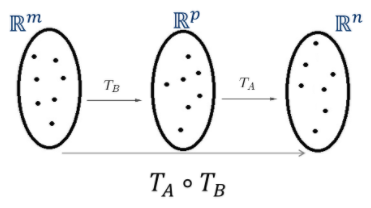
\includegraphics[scale=0.5]{comp-trans.png}
\end{center}

Would imply that $A$ is $n\times p$, $B$ is $p\times m$, and $AB$ is $n\times m$.
Can define the following:

\[\boxed{\text{The $i^{th}$ column of the matrix $AB$ is the matrix-vector product $A$($i^{th}$ column of the matrix $B$)}}\]

\subsection{Proofs}

\textbf{\textit{Claim:}} The product of 2 invertible matrices must be an invertible matrix.\newline
\textbf{\textit{Proof:}} Given that $(AB)(AB)^{-1}=I_n$:

\begin{align*}
    &(AB)(AB)^{-1}=I_n\\
    &A(B(AB)^{-1})=I_n\\
    &A^{-1}A(B(AB)^{-1})=A^{-1}I_n\\ 
    &B(AB)^{-1}=A^{-1}\\ 
    &B^{-1}B(AB)^{-1}=B^{-1}A^{-1}\\
    &(AB)^{-1}=B^{-1}A^{-1}
\end{align*}

\noindent\textbf{\textit{Claim:}} If $(AB)^{-1}$ exists, then $A$ and $B$ are both invertible.\newline
\textbf{\textit{Proof:}} Given that $(AB)(AB)^{-1}=I_n$ and $(AB)^{-1}(AB)=I_n$:

\begin{align*}
    &A(B(AB)^{-1})=I_n\\ 
    &((AB)^{-1}A)B=I_n\\
    &\boxed{\therefore\;\exists\;A^{-1},\:B^{-1}\in \R^n}
\end{align*}

\subsection{Properties}

\begin{itemize}
    \item Associativity: $(AB)C=A(BC)$
    \item Distribution: $A(B+C)=AB+BC$
    \item Respects scalar multiplication: $(kA)B=k(AB)=A(kB)$ 
\end{itemize}
